\normalfalse \difficiletrue \tdifficilefalse
\correctiontrue

%\UPSTIidClasse{12} % 11 sup, 12 spé
%\newcommand{\UPSTIidClasse}{12}

\exer{Mouvement RT -- RSG  $\star\star$ \label{C1:05:46}}
\setcounter{question}{0}\UPSTIcompetence[2]{B2-14}
\UPSTIcompetence[2]{C1-05}
\index{Compétence B2-14}
\index{Compétence C1-05}
\index{Principe fondamental de la dynamique}
\index{PFD}
\index{Mécanisme 2 rotations et RSG}
\index{Culbuto}
\ifcorrection
\else
\marginnote{\textbf{Pas de corrigé pour cet exercice.}}
\fi

\ifprof
\else
Soit le mécanisme suivant. On a $\vect{IA}=R\vect{j_0}$ et $\vect{AB}=L\vect{i_2}$. De plus $R=\SI{15}{mm}$.
On fait l'hypothèse de roulement sans glissement au point $I$. De plus :
\begin{itemize}
\item $G_1$ désigne le centre d'inertie de \textbf{1} tel que $\vect{AG_1}=-\ell\vect{i_1}$, on note $m_1$ la masse de \textbf{1};% et $\inertie{G_1}{1}=\matinertie{A_1}{B_1}{C_1}{0}{0}{0}{\bas{1}}$; 
\item $G_2=B$ désigne le centre d'inertie de \textbf{2}, on note $m_2$ la masse de \textbf{2}.% et $\inertie{G_2}{2}=\matinertie{A_2}{B_2}{C_2}{0}{0}{0}{\bas{2}}$.
\end{itemize}
Un moteur exerce un couple entre les pièces 1 et 2. 
\begin{center}
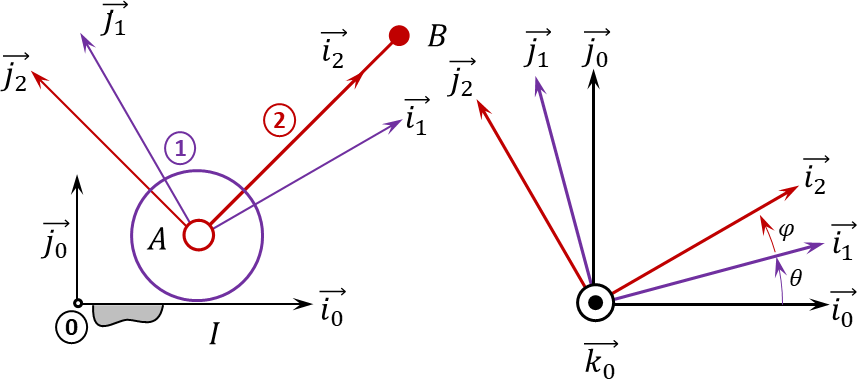
\includegraphics[width=\linewidth]{01}
\end{center}
\fi

\question{Réaliser le graphe d'analyse en faisant apparaître l'ensemble des actions mécaniques.}
\ifprof
\begin{center}
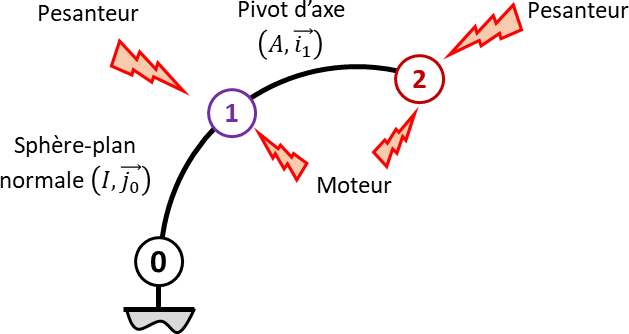
\includegraphics[width=\linewidth]{46_01_cor}
\end{center}

\else
\fi

\question{Proposer une démarche permettant de déterminer les loi de mouvement de \textbf{1} et de \textbf{2} par rapport à~$\rep{0}$.}
\ifprof

\begin{itemize}
\item Première équation : 
\begin{itemize}
\item On isole 2.
\item Bilan des actions mécaniques extérieures :
\begin{itemize}
\item liaison pivot en $A$ telle que $\vectm{A}{1}{2}\cdot \vect{k_0} = \vect{0}$;
\item pesanteur en $B$ : $\torseurstat{T}{\text{pes}}{2} = \torseurl{-m_2 g \vect{j_0}}{\vect{0}}{B}$;
\item cople moteur : $\torseurstat{T}{1_m}{2} = \torseurl{\vect{0}}{C_m\vect{k_0}}{\forall P}$.
\end{itemize}
\item On applique le théorème du moment dynamique en $A$ en projection sur $\vect{k_0}$.
\end{itemize}
\item Deuxième équation : 
\begin{itemize}
\item On isole 1+2.
\item Bilan des actions mécaniques extérieures :
\begin{itemize}
\item liaison ponctuelle avec RSG en $I$ telle que $\vectm{I}{0}{1}\cdot \vect{k_0} = \vect{0}$; 
\item pesanteur en $G_1$  : $\torseurstat{T}{\text{pes}}{1} = \torseurl{-m_1 g \vect{j_0}}{\vect{0}}{G_1}$;
\item cople moteur : $\torseurstat{T}{2}{1_m} = \torseurl{\vect{0}}{-C_m\vect{k_0}}{\forall P}$.
\end{itemize}
\item On applique le théorème du moment dynamique en $I$ en projection sur $\vect{k_0}$.
\item Remarque : on ne modélise pas la résistance au roulement. 
\end{itemize}

\end{itemize}
\else
\fi



\ifcolle
\question{Déterminer les lois de mouvement.}
\else
\fi

\ifprof
\else
\begin{flushright}
\footnotesize{Corrigé  voir \ref{C1:05:46}.}
\end{flushright}%
\fi